\documentclass{article}
\usepackage[utf8]{inputenc}
\usepackage{setspace}
\usepackage{graphicx}
\usepackage{dirtree}
\usepackage{placeins}
\usepackage[hang]{footmisc}
\usepackage{vhistory}
\usepackage{tikz}
\usetikzlibrary{shapes.geometric, arrows}
\renewcommand{\hangfootparskip}{10pt}
\setlength{\skip\footins}{1cm}
\setlength{\parskip}{1em}
\usepackage[a4paper, total={6in, 8in}]{geometry}



\title{%
Lustre Low Level Design \\
\large Zenuity Oden Cluster (NGSC)}
\author{Carlos Thomaz - cthomaz@ddn.com}
\date{\today}
\begin{document}

\maketitle


\begin{center}
    
\includegraphics[scale=0.14]{logo.png}\\[1cm] 
\end{center}
\begin{center}
version 1.1
\end{center}

\newpage

\begin{versionhistory}
    \vhEntry{Draft}{06.05.2020}{CT}{Initial version}
    \vhEntry{Draft}{06.14.2020}{CT}{v1.1 - fixes and section 4.9.1 added}


\end{versionhistory}
\newpage

\tableofcontents

\newpage
\section{Introduction}
The goal of this document is to describe the Lustre File System low level design to be implemented at Zenuity's Oden cluster. The document provides details on how the overall design of multiple firezones and namespaces were architected and references other documents that has details about critical aspects of the system that has been previously discussed with HPE and Zenuity team.

\section{System Architecture - High Level}
Zenuity's Oden cluster is architected to provide isolation and reliability across multiple cells, also known as firezones. Each firezone could be considered a self contained cluster with computer, network and storage resources. End users will have access to the multiple firezones according to the access policies to be established prior the production rollout. The firezones will not be installed nor deployed all at once. Instead, they will be rolled out sequentially over the next months according to the computational demand. A total of six firezones are initially expected. 

\begin{figure}[h]
    \centering
    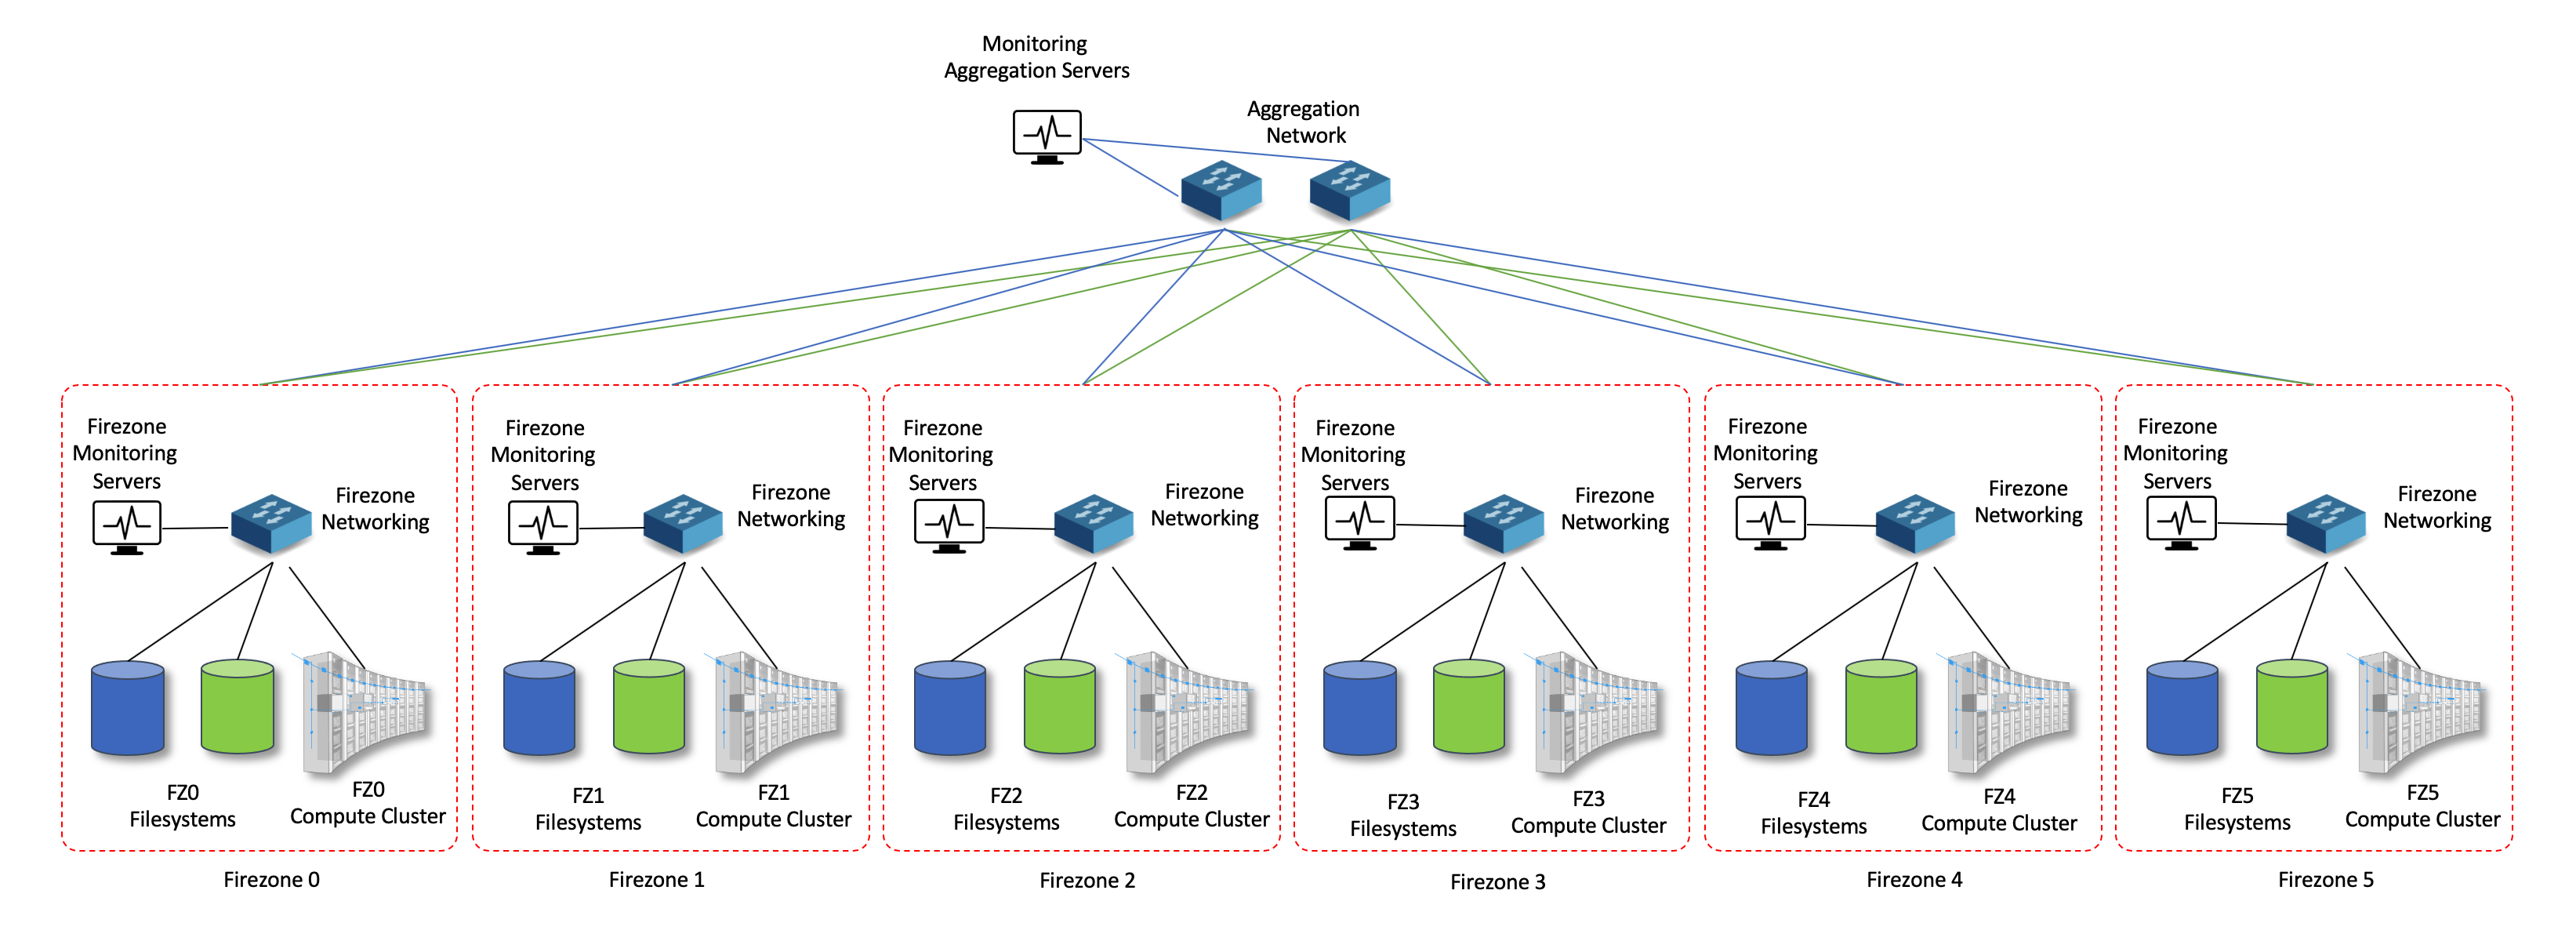
\includegraphics[scale=0.26]{Firezones-high-level.png}
    \caption{High Level view of Oden's firezones}
    \label{fig:firezones-general-view}
\end{figure}

\subsection{Firezones}
As mentioned before, each firezone is a self contained cell of computers, network and storage resources. Each firezone will be provided with redundancy and fault resilience that includes two independent filesystems (namespaces) that will server the firezone's computer clients. 

Each firezone is subjected to grow over time and filesystems will be expanded according to the capacity's demand. The filesystem growth will be triggered by pre-defined criterias, today set as \textbf{capacity}, but not limited to. 

These namespaces are based on DDN's Exascaler, a Lustre parallel file system implementation based on DDN SFA storage building blocks.

\subsection{Lustre file system namespaces}
As mentioned before, each firezone will be provided with two independent namespaces. Each namespace will be capable to grow and expand its capacity and performance according to the computational demand to be observed after the initial project rollout. It is Zenuity's decision to increase or not the capacity of each filesystem. The overall architecture predicts a 4x fold capacity increase per filesystem, per firezone. However, additional scalability is possible and if necessary will can be discussed further.

\subsubsection{Filesystem Building Blocks}
Each Firezone will host two independent filesystem namespaces. These namespaces are based on Lustre parallel file system that requires different hardware components (Scalable units). This session explain in more details the Filesystem Building Block. 

Filesystem Building Blocks is referred in this context to a \textbf{a set of hardware and software components that builds a fully functional Lustre File System namespace as well the set of components used to grow this file system in the future}. It is called Lustre Component Building Blocks the elements that are required to build a lustre file system.
\begin{figure}[h]
    \centering
    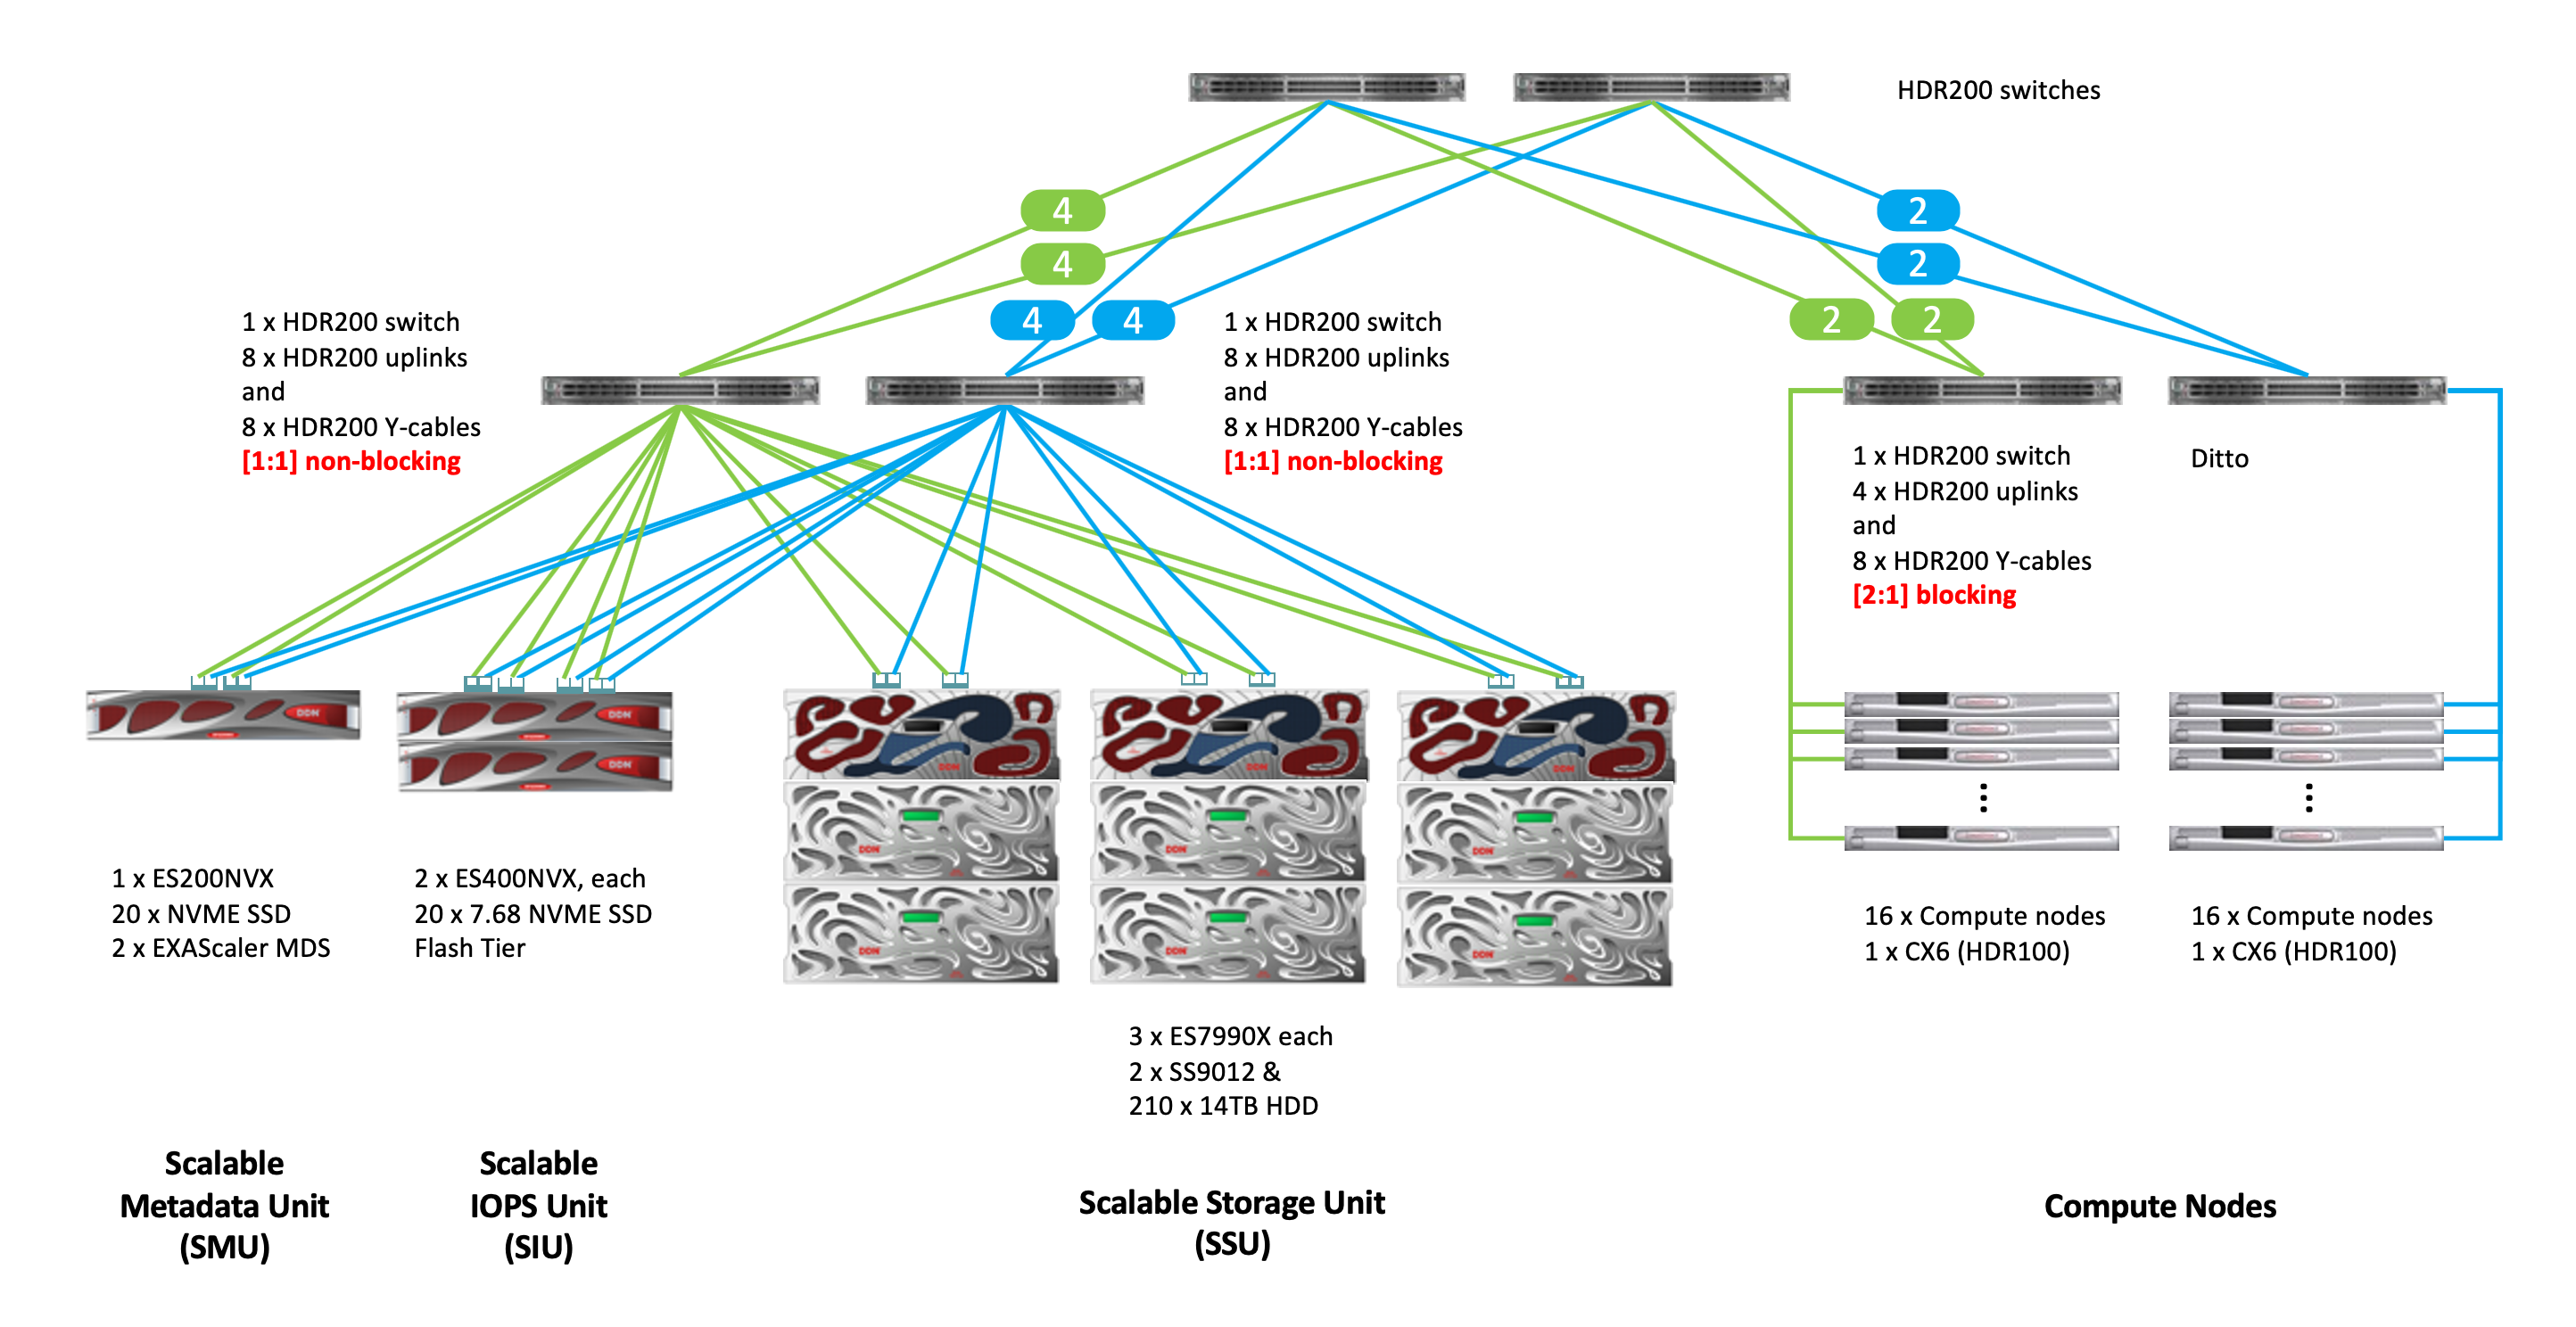
\includegraphics[scale=0.30]{Zenuity-Building-block.png}
    \caption{Zenuity - Oden File System Building Block}
    \label{fig:zenuity-lustre-block}
\end{figure}

Oden's Lustre file system architecture relies on \textbf{Scalable Metadata Units - SMU}, \textbf{Scalable IOPS units (SIU)}, \textbf{Scalable Storate Unit (SSU)}, and a high speed network fabric that connects all the components and its clients.

SMU are known as Lustre Metadata Servers. It provides the index, or namespace, for a Lustre file system. The metadata content is stored on volumes called Metadata Storage Targets (MDTs). A Lustre file system’s directory structure and file names, permissions, extended attributes, and file layouts are recorded to the MDTs. Each Lustre file system must have a minimum of one MDT, which contains the root of the file system namespace, but a single Lustre file system can have many MDTs for file systems with complex directory structures and very large quantities of files.

SIU and SSU are known as Lustre Object Storage Servers. The Object Storage Servers (OSS) in a Lustre file system provide the bulk data storage for all file content. Each OSS provides access to a set of storage volumes referred to as Object Storage Targets (OSTs) and each object storage target contains a number of binary objects representing the data for files in Lustre.

Oden's filesystems building blocks has two different types of Lustre OSS. The SIU and SSU defining two object tiers in the same file system. The devices and storage controllers are different on SIU and SSU. SIU are designed for IOPS and potentially smaller and more transactional I/O workloads while SSU are designed for large sequential bulk I/O workloads.

\subsubsection{Scalable Metadata Unit - SMU}
Each namespace will be provided with one SMU. The initial design doesn't consider the expansion of multiple SMUs in a single file system, although Lustre file system architecture allows to grow it, if necessary. 

The SMU is based on the DDN ES200NVX platform, an appliance built on top of fully redundant platform that holds two DDN SFA RAID controllers and 20 (twenty) Non-volatile Memory modules. This scalable units are designed to handle high metadata workloads. 

The ES200NVX controllers will host two Lustre Metadata Servers and requires only two rack units of space, providing 150K file creates per second. It also provides fully redundant components such as management and Infiniband host devices.

\begin{figure}
    \centering
    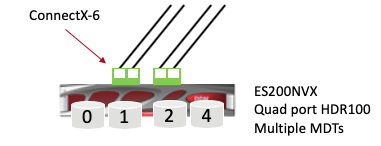
\includegraphics[scale=0.60]{SMU.png}
    \caption{Scalable Metadata Unit - SMU}
    \label{fig:smu}
\end{figure}

The SMU will also host the Lustre Management Server (MGS) that is a necessary component for each namespace. It is required one MGS and MGT (Lustre Management Target) per namespace.

\subsubsection{Scalable IOPS Unit - SIU}
Aiming to reduce latency and improve small and transactional I/O worklaods a NVME based Object Storage unit (SIU) has been designed and will be implemented on each filesystem namespace. 

The SIU is composed by two DDN ESN400VX with a total of 40 Non-volatile memory modules, NVMEs, configured as Lustre Object Storage server unit. As the SMU, these modules are fully redundant without single point of failure. Each ES400NVX will host 4 (four) Lustre OSSs. 

\begin{figure}
    \centering
    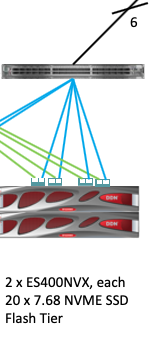
\includegraphics[scale=0.50]{SIU.png}
    \caption{Scalable IOPS Unit - SIU}
    \label{fig:SIU_block}
\end{figure}

\subsubsection{Scalable Storage Unit - SSU}
The largest set of data will be hosted on the Scalable Storage Units, Lustre Object Storage Servers based on DDN ES7990X appliances provided with standard Rotational devices (HDD). 

The majority of each namespace capacity is provided by these scalable units. Possible upgrades are designed to scale adding SSUs, thus increasing the capacity and performance of an existing filesystem.

The initial design considers three DDN ES7990X, each one with a total of 210 HDDs and aggregating 50GB/sec of peak performance (Bulk sequential I/O).

\begin{figure}
    \centering
    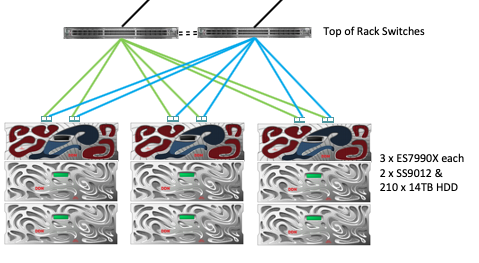
\includegraphics[scale=0.50]{SSU.png}
    \caption{Scalable Storage Unit - SSU}
    \label{fig:SSU_block}
\end{figure}

The SSUs will require a total of 36 Rack Units.

\subsubsection{Monitoring Services}
Monitoring Services will be deployed on each firezone. Two DDN Insight Servers will be properly configured (one per filesystem) providing filesystem performance monitoring statistics. 

These statistics can be gathered by filesystem but also will be, in the future, aggregated on a single dashboard where users and systems administrators will be able to monitor all namespaces through a single, aggregated dashboard. 

This document does not describes the Low level design of monitoring services

\subsubsection{Configuration and Deployment Manager services}
Single instances of configuration and deployment manager services will be installed system-wise, meaning, one single instance capable to manage and configure all file systems and namespaces residing on any firezones.

The configuration manager (CM) and Deployment Manager (DM) services will be installed and customized on the same hardware as the Insight Aggregation services that will have access to the common management network VLAN, which is the same for all firezones. From these instances, system administrators will be able to configure and manage multiple Lustre namespaces. Configuration Manager is discussed in details in a separated chapter.

\subsection{Rack Layouts}
Each namespace will be configured in two or more racks, depending on the number of expansions added in the future. The two initial racks will be divided by functional scalable units. The first rack will be dedicated to SIU and SMU (plus possible servers such DDN Insight Servers) and the second rack will be dedidated to the SSU expansions.

\subsubsection{Utility and Network Rack: Metadata and Flash Tier}
The first rack will be configured with the Metadata (SMU) and flash tier (SIU), and will provide space for further upgrades, if needed, or additional devices not considered in the initial project's design phase. It is mandatory to be installed as the rack elevation for organizational purposes. 

\begin{figure}[h]
    \centering
    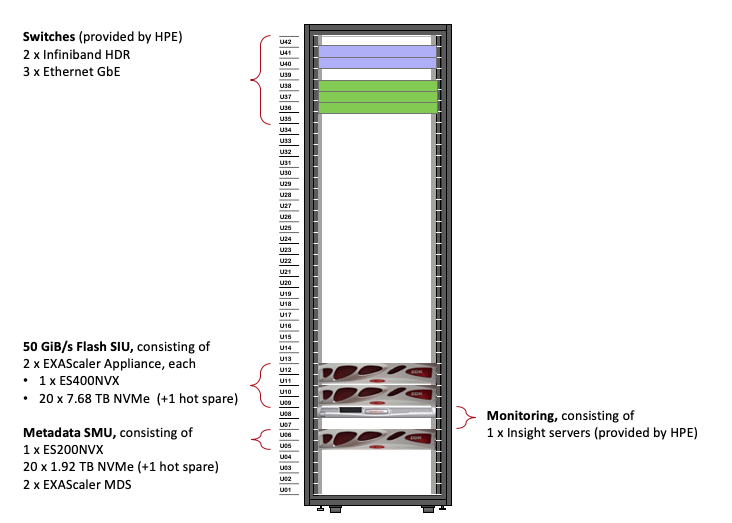
\includegraphics[scale=0.35]{utility-rack.png}
    \caption{Utility and Network Rack}
    \label{fig:util-rack}
\end{figure}

\subsubsection{Storage Scalable Unit Rack}
The second and subsequent racks will be configured with the SSU (Lustre OSSs) which represents the rotational device and capacity tier of each namespace. Additional expansions will be deployed adding a minimum of a rack. 

\begin{figure}[h]
    \centering
    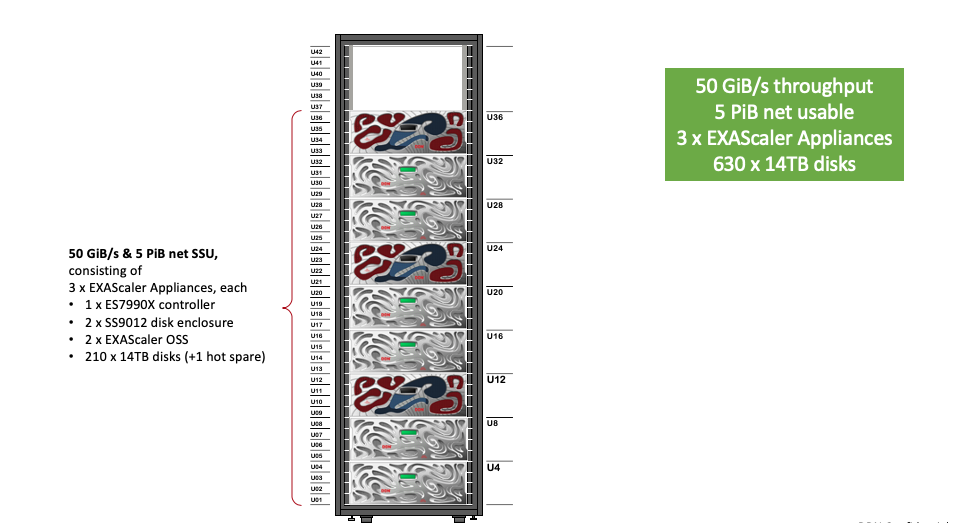
\includegraphics[scale=0.35]{SSU-rack.png}
    \caption{Storage Scalable Unit Rack}
    \label{fig:SSU-rack}
\end{figure}

\subsubsection{Namespace and Expansions}
A namespace within a firezone is expected to grow up to four times, capacity and performance-wise (considering the same HDD capacity and technology). A potential 20PiB and 200GB/sec per namespace is expected during the course of the project. The rack elevation layout for a namespace in its full capacity is demonstrated on Figure \ref{fig:namespace-full}.

\begin{figure}[h]
    \centering
    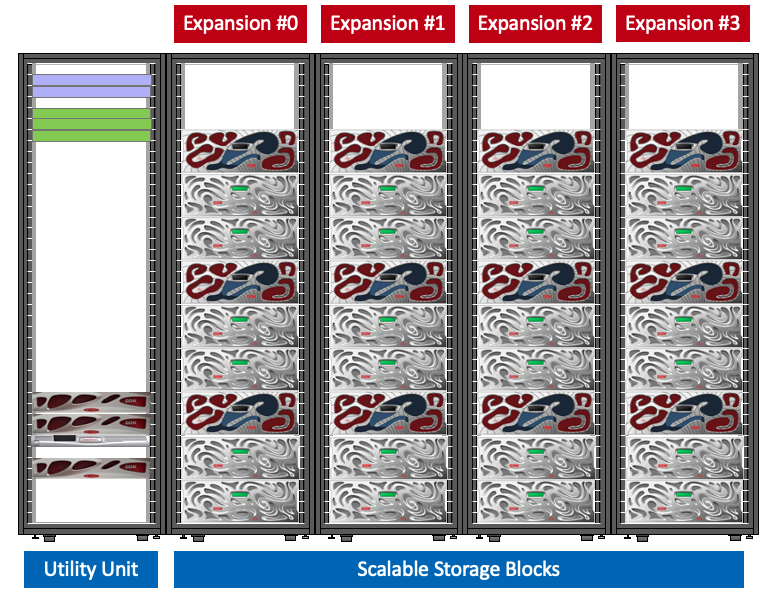
\includegraphics[scale=0.30]{full-namespace.png}
    \caption{A namespace with all potential expansions}
    \label{fig:namespace-full}
\end{figure}

\subsubsection{Firezone - Namespaces}
Once expanded and its full capacity a firezone will host a total of 10 racks totalizing 400GiB/sec and 40PiB of NET capacity distributed in two even namespaces. The storage rack elevation is illustrated on Figure \ref{fig:firezone-full}.

\begin{figure}[h]
    \centering
    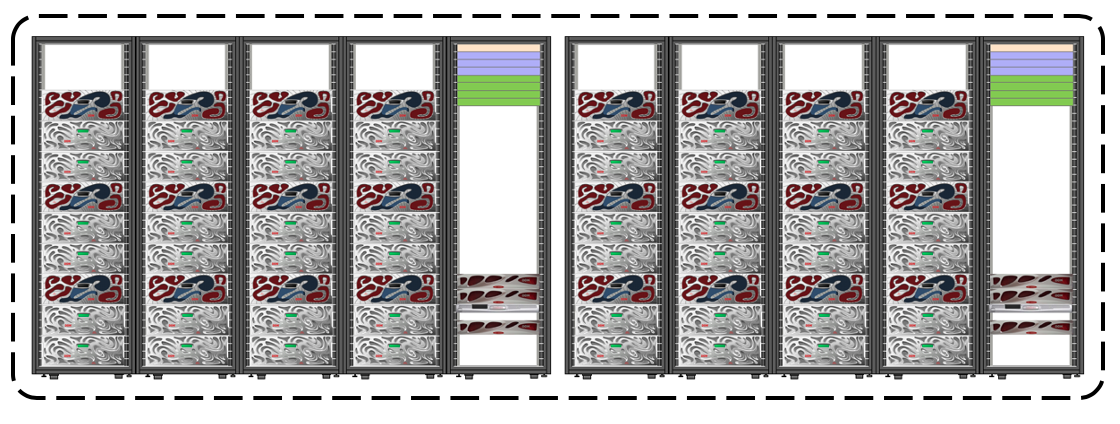
\includegraphics[scale=0.30]{full-firezone.png}
    \caption{Storage Rack elevation of a fully deployed firezone}
    \label{fig:firezone-full}
\end{figure}
\FloatBarrier

\newpage
\section{Lustre File System - Low Level Design (SOFTWARE)}
DDN Exascaler is a full stack software that combines the Lustre File System implementation with a set of of other tools and frameworks required to provide a highly available and easily managed parallel file system solution. 

This section describes the low level design and how DDN Exascaler will be implemented on each namespace within each firezone based on the hardware architecture described on the previous sections of this document.

Each namespace will be configured similarly and it is not expected significant differences between different namespaces. It is under consideration the version leveling as well a homogeneous implementation of all parameters on each namespace. Ideally, all namespaces should behave identically and DDN will enforce the parametrization is identical across all firezones. 

\subsection{Naming convention}
A common naming convention has been defined and will be used on all deployed systems. This section explains in general terms the naming convention used to the major components in the system.

\subsubsection{Hostnames}
Virtual servers or SFA controllers (and any other component that has an addressable IP address) shall have a canonical name assigned to. These names follows the mnemonic explained below:
\begin{center}
    $$
    \underbrace{se01}_{Location}\underbrace{z01}_{Firezone}\underbrace{sfa100}_{type}
    $$
\end{center}

\begin{table}[htbp]
\resizebox{\columnwidth}{!}{
\begin{tabular}{|l|l|l|}
    \hline
    se01 & Physical site & refers to the system installed in a specific datacenter (e.g. Digiplex)  \\
    z01 & Firezone & refers to the firezones within that datacenter \\
    sfa & Component & Equipment type or host \\
    100 & sequence number & three digit unique integer \\
    \hline
\end{tabular}}
\caption{Naming convention for hostnames and component names }
\label{tab:naming-hostnames-table}
\end{table}

The type of entities could either be \textit{sfa}, \textit{mds}, \textit{oss}.
Additional identifiers may be required in certain contexts. For instance, \textit{-zN} (where N is an integer) can be used to identify a controller member in sfa devices. For instance, se01z01sfa100-\textbf{z1} may refer to one controller that is a member of SFA storage 100. Other identifiers may be used as well, such as \textit{-ib0} or \textit{-ipmi} to identify the type of interface to be addressed.

\subsection{SMU - Lustre Metadata Services}
As explained previously Lustre Metadata Services will run on specific hardware designed for this purpose. The ES200NVX is configured with 20 NVMe devices that will be properly partitioned and configured as Metadata Targets (MDTs). 

\subsubsection{Physical Configuration - Pools and VDs}
The ES200NVX will be configured with a single DCR (De-clustered RAID) pool with minimum rebuilds set to 0 and type HPC. This pool will be built on top of all 20 available devices. 

Four VDs (Virtual Disks) will be then created on top of the DCR pool. The pool assignment is defined on the table below.

\begin{table}[htbp]
\resizebox{\columnwidth}{!}{
\begin{tabular}{|l|l|l|l|l|l|}
    \hline
    \textbf{VD Index} & \textbf{VD Name} & \textbf{RAID Level} & \textbf{Chunk Size} & \textbf{Capacity} & \textbf{Utilization}\\
    \hline
    0 & zds10-mdt0000\_s0 & raid6 & 128Kb & 8TiB & Lustre Metadata Target\\
    1 & zds10-mdt0001\_s0 & raid6 & 128Kb & 8TiB & Lustre Metadata Target\\
    100 & mgs & raid 1 & default & min\_capacity & Lustre management server target\\
    101 & mgs\_backup & raid 1 & default & 14796GiB & MGS backup \\
    \hline
\end{tabular}}
\caption{ES200NVX Disk Pools and Virtual Disks}
\label{tab:es200-pools-vds-table}
\end{table}

The \_s0 are required by DDN Exascaler naming of Metadata Targets. It is used internally and it is inherited and preserved for backwards compatibility. 

\subsection{SIU - Lustre Object Storage Services, IOPS}
The SIU storage (IOPS driven configuration) will be configured similarly using DDN ES400NVX storage modules. There are total of 2 (two) ES400NVX storage modules, each one with two embedded virtual OSS servers configured.

\subsubsection{Physical Configuration - Pools and VDs}
Each ES400NVX will be configured with 2 (two) DCR pools, each containing 10 NVMe devices, with minimum rebuilds set to 0 and type set to HPC. 

\begin{table}[htbp]
\centering
\begin{tabular}{|l|l|l|l|l|l|}
    \hline
    \textbf{Pool Index} & \textbf{Pool Name} & \textbf{Minimum Rebuilds} & \textbf{Type} & \textbf{Number of PDs}\\
    \hline
    0 & zds10\_ost\_0 & 0 & HPC & 10 \\
    1 & zds10\_ost\_1 & 0 & HPC & 10 \\
    \hline
\end{tabular}
\caption{ES400NVX Disk Pools}
\label{tab:es400-pools-table}
\end{table}

Eight Virtual Disks (VDs) will be created on each ES400NVX. They will be spread out evenly on two DCR pools as follow.

\begin{table}[htbp]
\resizebox{\columnwidth}{!}{
\begin{tabular}{|l|l|l|l|l|l|}
    \hline
    \textbf{VD Index} & \textbf{VD Name} & \textbf{RAID Level} & \textbf{Chunk Size} & \textbf{Capacity} & \textbf{Utilization}\\
    \hline
    0 & zds10\_ost0000 & raid6 & 128Kb & 14240GiB & Lustre Object Storage Target\\
    1 & zds10\_ost0001 & raid6 & 128Kb & 14240GiB & Lustre Object Storage Target\\
    2 & zds10\_ost0002 & raid6 & 128Kb & 14240GiB & Lustre Object Storage Target\\
    3 & zds10\_ost0003 & raid6 & 128Kb & 14240GiB & Lustre Object Storage Target\\
    4 & zds10\_ost0004 & raid6 & 128Kb & 14240GiB & Lustre Object Storage Target\\
    5 & zds10\_ost0005 & raid6 & 128Kb & 14240GiB & Lustre Object Storage Target\\
    6 & zds10\_ost0006 & raid6 & 128Kb & 14240GiB & Lustre Object Storage Target\\
    7 & zds10\_ost0007 & raid6 & 128Kb & 14240GiB & Lustre Object Storage Target\\
    
    \hline
\end{tabular}}
\caption{ES400NVX Virtual Disks}
\label{tab:es200-vds-table}
\end{table}

The indexes numbers are unique \textbf{within} each SFA storage module. So, it is expected that each ES400NVX to have Pool indexes varying from 0 to 1 and VD indexes varying from 0 to 7. However, the VD name (translated into OST device name) shall be sequentially assigned and unique across the namespace.

Exascaler assumes the OST names to use the following mnemonic: \textit{filesystem-name}\_\textit{OST-numbering}.

\subsection{SSU - Lustre Object Storage Services}
The SSU storage (Capacity driven configuration) is designed based on rotational Hard Disk drives. The DDN storage module to be deployed as SSU is the DDN ES7990 with two expansion units providing a maximum expansibility of 270 slots. A total of 210 slots are populated with 14TB 7200RPM NL-SAS devices. 

A total of 3 (three) ES7990X will be initially deployed. Additional expansions may be added into the configuration where each building block will be composed by a rack fully loaded (correspondent to three ES7990X). 

Each ES7990X will be configured with 2 (two) virtual Lustre Object Storage Servers (OSS).

\subsubsection{Physical Configuration - Pools and VDs}
Each ES7990X will be configured with 6 pools, each one containing 35 physical disks (PDs). Six VDs will be created using the entire capacity of the pools. 

\begin{table}[htbp]
\centering
\begin{tabular}{|l|l|l|l|l|l|}
    \hline
    \textbf{Pool Index} & \textbf{Pool Name} & \textbf{Minimum Rebuilds} & \textbf{Type} & \textbf{Number of PDs}\\
    \hline
    0 & zds10\_ost\_0016 & 0 & HPC & 10 \\
    1 & zds10\_ost\_0017 & 0 & HPC & 10 \\
    2 & zds10\_ost\_0018 & 0 & HPC & 10 \\
    3 & zds10\_ost\_0019 & 0 & HPC & 10 \\
    4 & zds10\_ost\_0020 & 0 & HPC & 10 \\
    5 & zds10\_ost\_0021 & 0 & HPC & 10 \\
    \hline
\end{tabular}
\caption{ES7990X Disk Pools}
\label{tab:es7990x-pools-table}
\end{table}

\begin{table}[htbp]
\resizebox{\columnwidth}{!}{
\begin{tabular}{|l|l|l|l|l|l|}
    \hline
    \textbf{VD Index} & \textbf{VD Name} & \textbf{RAID Level} & \textbf{Chunk Size} & \textbf{Capacity} & \textbf{Utilization}\\
    \hline
    0 & zds10\_ost0016 & raid6 & 256Kb & Max & Lustre Object Storage Target\\
    1 & zds10\_ost0017 & raid6 & 256Kb & Max & Lustre Object Storage Target\\
    2 & zds10\_ost0018 & raid6 & 256Kb & Max & Lustre Object Storage Target\\
    3 & zds10\_ost0019 & raid6 & 256Kb & Max & Lustre Object Storage Target\\
    4 & zds10\_ost0020 & raid6 & 256Kb & Max & Lustre Object Storage Target\\
    5 & zds10\_ost0021 & raid6 & 256Kb & Max & Lustre Object Storage Target\\
    \hline
\end{tabular}}
\caption{ES7990X Virtual Disks}
\label{tab:es7990x-vds-table}
\end{table}
The Virtual Disks will be set to the maximum capacity allowed.

\section{Exascaler - Global Configurations}
Exascaler requires design decision about global configuration options. For management purposes DDN suggests to keep most of the configurations identical, replacing only the variables that are unique for each namespace as names, IP addresses and other variables subjected to be unique per namespace and firezones.

\subsection{Filesystems and Namespaces}
Each building block (a set of SMU, SIU and SSU) will host \textbf{only} one (1) namespace. Although Exascaler provides the capability of having multiple namespaces running in the same hardware set, a design decision has been taken to only host one file system per hardware building block, so the Lustre MGS will be only managing a single namespace. 

The filesystem name is identified by \textbf{\textit{identificationXX}} where the \textit{identification} is a string and \textit{XX} is a two-digit integer. The file system name \textbf{MUST BE} unique across the entire infra-structure and can't expand more than eight digits.

\subsection{Timezone}
\textbf{UTC} will be set for all namespaces within the Oden Cluster.

\subsection{High Availability}
DDN Exascaler relies on Linux HA framework to provide highly available services. Exascaler implements \textit{Corosync} as cluster messaging layer and will be configured in conjunction of Linux Pacemaker as resource manager.

Each DDN storage module will be deployed with 2 (two) or 4 (four) embedded virtual servers. This server pair will be configured as a self-contained HA pair with access with the same shared storage resources. These two virtual servers, in the context of Linux HA, will be defined as one \textit{HA group}. 

The SMU and SSU (Metadata and Object Storage Unit), repectively based on DDN ES200NVX and ES7990X will be configured with one virtual VM per controller, or two virtual machines per system, while the ISU, based on ES400NVX, will be deployed with four virtual machines for maximum performance. 

Each HA pair requires a shared storage for resource failover purposes. The storage will be evenly balanced under normal operation, with the same number of resources evenly distributed. 

A total of 17 HA groups will be configured in the initial deployment of a namespace, with potential 18 HA groups to be added in the future with further expansions. 

\subsubsection{HA settings and requirements}
Linux HA requires pre-requisites to operate in its fully redundant way. At least one external management network, also known as Corosync Ring, is necessary for HA cluster communication. All internal Corosync and Pacemaker communication will happen using the corosync rings. In order to increse the availability and remove single point of failures, two corosync rings will be established on each HA cluster.

\begin{table}[htbp]
\centering
\begin{tabular}{|l|l|l|}
    \hline
    \textbf{Ring} & \textbf{Physical Interface} & \textbf{Type}\\
    \hline
    ring0 & enp3s0 & Ethernet \\
    ring1 & ib0 & Infiniband \\
    \hline
\end{tabular}
\caption{Exascaler Corosync Rings}
\label{tab:es-corosync-rings}
\end{table}

HA interprocesses communication will use the unicast and passive redundant ring protocol. 
Below is the list of HA groups and server peers for a initial cluster configuration (filesystem zds10).

\begin{table}[htbp]
\centering
\begin{tabular}{|l|l|l|l|}
    \hline
    \textbf{HA group} & \textbf{Peer 0} & \textbf{Peer 1} & \textbf{Type}\\
    \hline
    ha\_group0 & se01z01mds100 & se01z01mds101 & MDS servers - SMU \\
    ha\_group1 & se01z01oss100 & se01z01oss101 & OSS server - SIU\\
    ha\_group2 & se01z01oss102 & se01z01oss103 & OSS server - SIU\\
    ha\_group3 & se01z01oss104 & se01z01oss105 & OSS server - SIU\\
    ha\_group4 & se01z01oss106 & se01z01oss107 & OSS server - SIU\\
    ha\_group5 & se01z01oss108 & zse01z01oss109 & OSS server - SSU\\
    ha\_group6 & se01z01oss110 & se01z01oss111 & OSS server - SSU\\
    ha\_group7 & se01z01oss112 & se01z01oss113 & OSS server - SSU\\
    ha\_group8 & se01z01oss114 & se01z01oss115 & OSS server - SSU\\
    ha\_group9 & se01z01oss116 & se01z01oss117 & OSS server - SSU\\
    ha\_group10 & se01z01oss118 & se01z01oss119 & OSS server - SSU\\
    ha\_group11 & se01z01oss120 & se01z01oss121 & OSS server - SSU\\
    ha\_group12 & se01z01oss122 & se01z01oss123 & OSS server - SSU\\
    ha\_group13 & se01z01oss124 & se01z01oss125 & OSS server - SSU\\
    ha\_group14 & se01z01oss126 & se01z01oss127 & OSS server - SSU\\
    ha\_group15 & se01z01oss128 & se01z01oss129 & OSS server - SSU\\
    ha\_group16 & se01z01oss130 & se01z01oss131 & OSS server - SSU\\
    \hline
\end{tabular}
\caption{Exascaler HA groups}
\label{tab:es-ha-groups}
\end{table}

\subsection{Storage Target Resources}
The system has two type of Storage Targets: Metadata Storage Targets (MDT) and Object Storage Targets (OST). Each namespace has only one MDS server pair and a total of two Metadata Targets. 

MDTs will provide about 8TiB of usable capacity that is enough to support up to 16 billion inodes with minimal inode allocation. 

SSU OSTs will provide about 342TiB of usable capacity while the SIU OSTs (flash based OSTs) will provide around 14TiB. 

\subsubsection{Storage Targets allocation per HA group}
The table shows the MDT and OST allocation per HA group (in this case a virtual server pair). MDTs and OSTs can be failed over between nodes that belongs to the same HA group. 

\begin{table}[htbp]
\centering
\begin{tabular}{|l|l|l|}
    \hline
    \textbf{HA group} & \textbf{Peer 0} &  \textbf{Type}\\
    \hline
    ha\_group0 & zds10\_mdt000[0-1]\_s0 & MDT \\
    ha\_group1 & zds10\_ost000[0-3] & OST \\
    ha\_group2 & zds10\_ost000[4-7] & OST \\
    ha\_group3 & zds10\_ost000[8-11] & OST \\
    ha\_group4 & zds10\_ost000[12-15] & OST \\
    ha\_group5 & zds10\_ost000[16-21] & OST \\
    ha\_group6 & zds10\_ost000[22-27] & OST \\
    ha\_group7 & zds10\_ost000[28-33] & OST \\
    \hline
\end{tabular}
\caption{Exascaler Storage Target Allocation per HA group}
\label{tab:es-storage-alloc-hagroup}
\end{table}


\subsubsection{Distributed Namespaces}
By default Lustre will implement DNE (Distributed Namespace) where both MDTs are used concurrently and allows the utilization of metadata stripping controlled by the client. DNE improves performance allowing inodes under the same subdirectories to be allocated across multiple Metadata Targets. The maximum DoM file size is set to 64Kb. 

\subsubsection{Data on Metadata}
Lustre allows metadata targets to be allocated for data. This is called Data on Metadata. The current design doesn't consider data on metadata, but it could be used if necessary. DoM will provide better performance for small file operations with a cost of consuming additional space on MDTs thus reducing the inode allocation capacity. 

\subsection{OST pools}
Default OST pools will be created for easy management and proper utilization of OST resources. One generic OST pool will be created with all FLASH based OSTs and a second pool will be created with all ROTATIONAL devices OSTs. However, it is recommended leveraging additional OST pools for easy data management in case of expansions. It is recommended the creation of OST pools per building blocks (set of 3 x ES7990X appliances) to facilitate data management and data control when additional building blocks are added in the same namespace. The techniques and more detailed information is provided on separate documentation where Data allocation and rebalancing is discussed. 

\subsection{Lustre Quotas}
Lustre provides two types of quotas. Usual POSIX quotas style where groups and users are subjected to quotas for capacity and inode utilization and the so called Lustre Project Quotas or Directory Quotas, where it is possible to adjust utilization limits for Object Storage Targets. Both quotas will be enable, but not enforced until the initial deployment. 

\subsection{Directory Services}
Lustre support upcalls to external directory services such as NIS and LDAP. By default no upcalls will be configured so the file system will rely on standard, locally set, user and password files. This can be changed at anytime if required in the future.

\subsection{Lustre Tuning}
There are several Lustre tuning parameters that will affect performance but also will establish limits to the system avoiding possible conflicts and resource starvation. All th best practices will be deployed by default, but the system will be subjected to fine tuning adjustments before and during the initial deployment stages. 

\subsubsection{IO Size}
All namespaces will be configured to support up to 16MB bulk I/O issued on the client side. This enable, if a contiguous I/O is issued on the client side, a single RPC to handle up to 16MB of streaming data, optimizing sequential reads and writes. 

\subsubsection{Lustre checksums}
By default checksums are ENABLED. Checksums guards the system against network data corruption. By default Lustre will deploy \textit{adler32} algorithm for checksums.

\subsubsection{Lustre changelogs}
Lustre changelogs will be enable for proper integration with HSM resources (HPE DMF). The following changelog mask will be enabled.
\begin{verbatim}
    "CREAT MKDIR HLINK SLINK MKNOD UNLNK RMDIR RENME XATTR CLOSE TRUNC
    SATTR MTIME CTIME HSM MIGRT"
\end{verbatim}

\subsection{Other specific configuration}
Other specific and detailed configuration is provided on the DDN IPG (Installation Planing Guide) that is filled by namespace. Specific details such as IP addresses, hostnames, network configuration and other parameters are properly detailed by namespace implementation on its specific IPG. 

\subsubsection{Exascaler version}
The system is installed with Exascaler 5.1.0 the most updated version at the time this document has been written. A further upgrade to Exascaler 5.1.1 may be considered specially on the \textbf{Client} side. It is relevant to highlight that Lustre clients don't need, and usually don't match the server side version. Lustre clients are usually simpler and may require different patch sets causing a version mismatch when compared with server side. 

The current Exascaler version is detailed on the DDN Lustre Version Matrix document.

\end{document}